\label{sec:structure_factor}
Атомы решетки, взаимодействуя с рентгеновским излучением, рассеивают его.
Если в элементарной ячейке более одного атома, волны от разных атомов,
 интерферируя между собой, вносят вклад в общую картину рассеяния,
 ослабляя или усиливая ее.

 \begin{figure}[H]
   \centering
   \subfloat[]{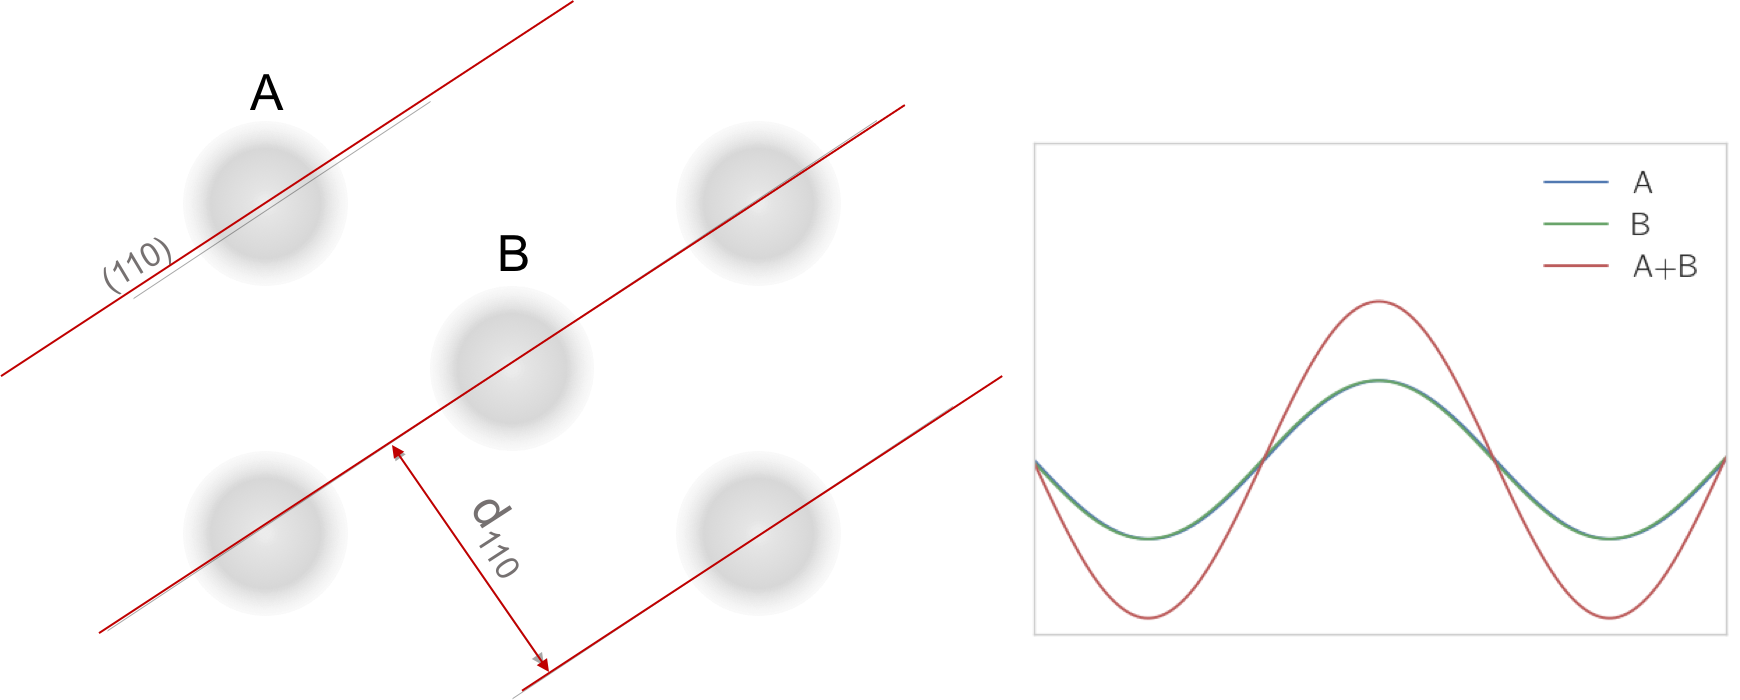
\includegraphics[width=0.45\textwidth]{images/interference_construct.png}}
   \hfill
   \subfloat[]{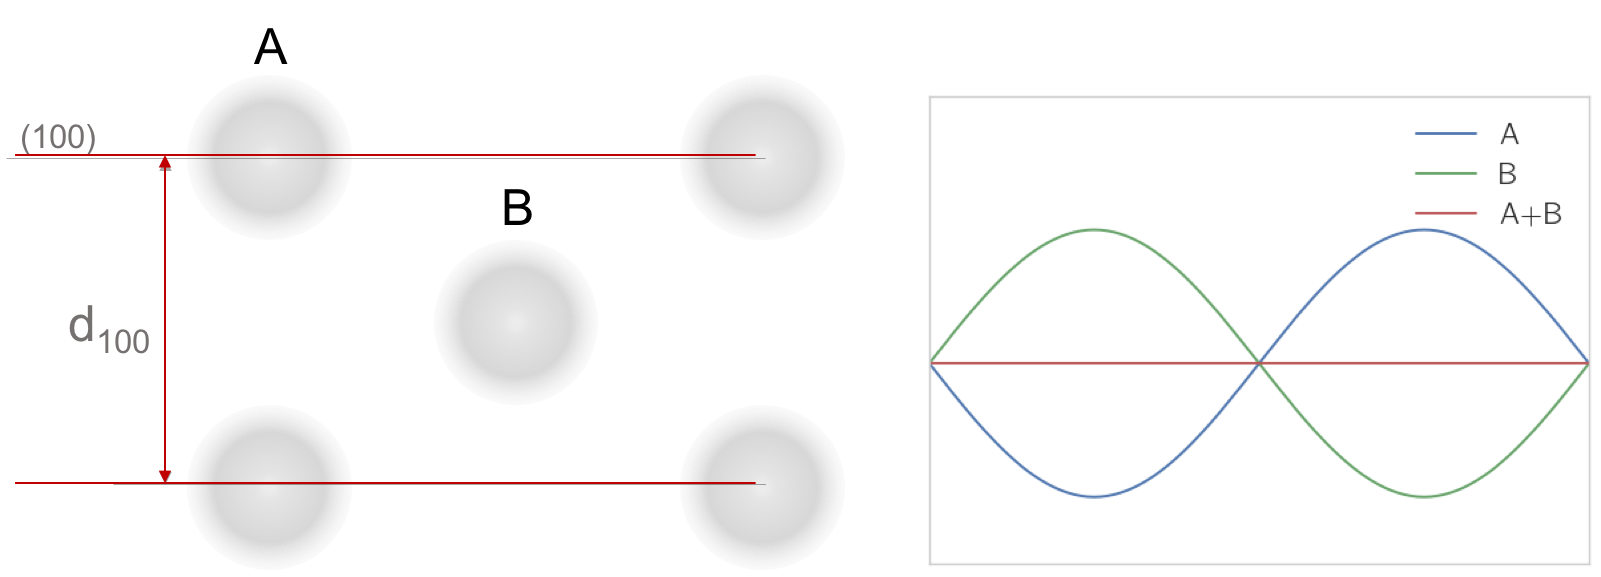
\includegraphics[width=0.45\textwidth]{images/interference_destruct.png}}
   \caption{Примеры интерференции двух волн, отраженных различными системами атомных плоскостей для случая
   конструктивной (a) и деструктивной (b) интерференции}
   \label{ris:interference_by_plate}
 \end{figure}

Рассеяние от набора атомов характеризуется структурным фактором, определяемым векторным
 сложением фаз по всем N атомам элементарной ячейки:

 \begin{equation}
   F = \sum_{n} f_n e^{ i\vec{h}\vec{r}_n} =   \sum_{n} f_n \cdot e^{-i\phi_n},
   \label{eq:F_factor}
  \end{equation}
\noindent
где $\phi_n = 2 \pi (hx_n+ky_n+lz_n)$;  $h, k, l$ - индексы Миллера; $x, y, z$ - относительные координаты
атомов в элементарной ячейке.

В соответсвии с \ref{eq:F_factor} в качестве примера был произведен расчет трехмерной ($hkl$) -
карты струкутрного фактора (рис. \ref{ris:hkl_LGT_SI}).
Цветом изображена величина структурного фактора для разных
 индексов плоскостей отражения для кристаллов LGT и Si.
 В таком представлении просматривается периодичность образования запрещенных
 рефлексов в кубическом кремнии. В кристалле LGT запрещенных (синий цвет)
  индексов для отражения на порядок меньше, связанно это с более низкой
  симметрией кристалла.

  \begin{figure}[h]
    \centering
    \subfloat[]{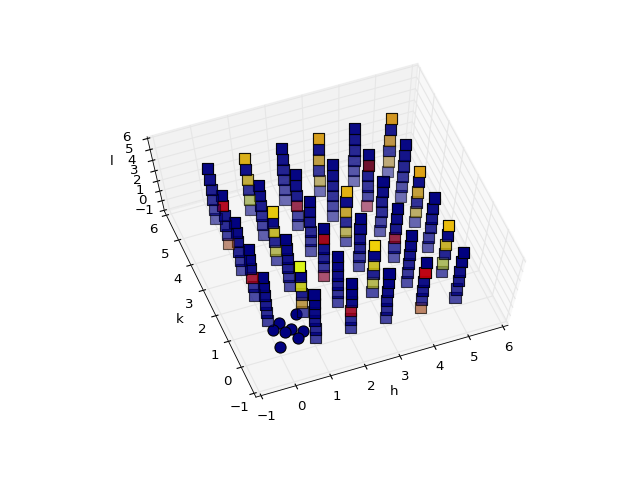
\includegraphics[width=0.5\textwidth]{images/hkl_Si.png} \label{ris:hkl_LGT_SI_a}}
    \hfill
    \subfloat[]{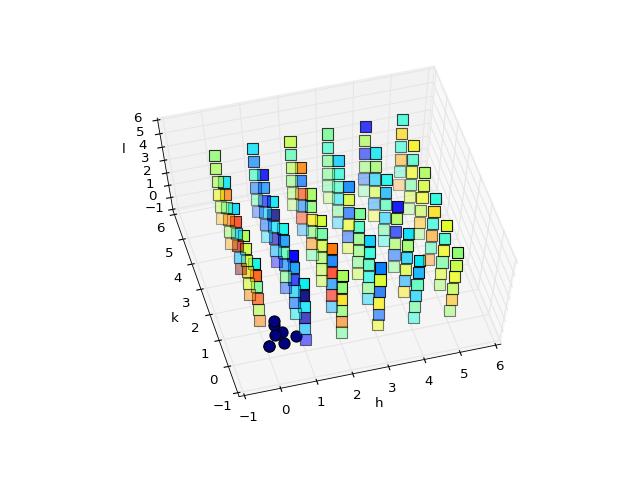
\includegraphics[width=0.5\textwidth]{images/hkl_LGT.png} \label{ris:hkl_LGT_SI_b}}
    \caption{Карта распределения величины структурного фактора
    (цвет соответствует его величине) в координатах индексов Миллера для кристалла Si (a) и LGT (b)}
    \label{ris:hkl_LGT_SI}
  \end{figure}
